\section{Columns and thin bands}\label{geo:section}

We first replace a plane graph by a family of vertical lines.  This separates
the length of a path from the planar restriction on its possible switches.
The replacement preserves the original metric exactly.  We then work in
a thin height band and prove two estimates for the later local updates:
entrances to a connected outer region lie near at most two fixed points,
and within each radial layer, connected groups of columns admit short
joining paths in the band.
All these estimates use the width of the band and the circular order of
the columns, with constants independent of their number.

\begin{definition}\label{geo:column-model}
A \emph{column model} consists of a finite cyclically ordered set $V_0$ of
indices, a copy $\{i\}\times\R$ of the height line for each $i\in V_0$, and
a finite collection of links.  A link $ij$ has a prescribed closed bounded
set $S_{ij}\subset\R$ of switch heights.  At $H\in S_{ij}$ we identify
$(i,H)$ with $(j,H)$.  The resulting quotient is denoted by $X$, and its
height function by $h$.  Paths consist of finitely many vertical segments
and permitted switches; their length is the sum of the lengths of the
vertical segments.  The distance $d$ is the infimum of these lengths.

The links are \emph{noncrossing} if no two have four distinct endpoints
alternating in the cyclic order.  We require all column models below to have
noncrossing links.  We additionally require that every link
between nonconsecutive indices is a switch at a single height $H_e$, and
that neither endpoint column has any switch above $H_e$.  Such a switch
will be called a \emph{terminal switch}.
Its quotient point is called the \emph{tip} of the link.

For a closed interval $I\subset\R$, possibly unbounded, write $X_I=h^{-1}(I)$.
The intrinsic distance $d_I$ only permits paths with heights in $I$;
different components have distance $+\infty$.  The active column graph
$G_I$ has vertex set $V_0$ and the links whose switch sets meet $I$ as edges.
\end{definition}

We write $B_{d_I}(x,r)$ for the closed ball and
$d_I(x,S)=\inf_{z\in S}d_I(x,z)$ for distance to a set, with
$d_I(x,\varnothing)=+\infty$. The same conventions apply to $d$.

\begin{lemma}[Realization and shortest paths]\label{geo:geodesics}
The function $d_I$ is a metric on each component of $X_I$.  Its finite
distances are attained by paths using each column at most once.  Components
of $X_I$ correspond exactly to components of $G_I$.  If $I$ is bounded, each
component of $X_I$ is compact.  For arbitrary $I$, bounded closed subsets of
each component are compact.  In particular distance from a point to a
nonempty compact set is attained.
\end{lemma}

\begin{proof}
If a path leaves a column and later returns to it, replace the intervening
part by the vertical segment joining its two visits.  This does not increase
length: total vertical variation is at least the difference of the two
heights.  The replacement stays in $I$.  Repeating the operation leaves
a path with no repeated column and at most $|V_0|-1$ switches.

There are finitely many possible such column words.  For a fixed word, its
switch heights belong to a product of closed bounded sets $S_{ij}\cap I$.
The length, including the initial and final vertical segments, is a
continuous function of these heights.  Thus every feasible word attains
its minimum, and minimizing over the finitely many words proves attainment.
A path of length zero has all its switches at the common endpoint height,
so its endpoints are already identified in the quotient.  This proves
positive definiteness.  The other metric axioms follow by reversing and
concatenating paths.

A permitted path projects to a walk in $G_I$.  Conversely any graph walk
can be realized by choosing an available height for each edge and moving
vertically between consecutive switches.  This proves the component claim.
The quotient map from any bounded closed piece of a column to $X_I$ is
$1$-Lipschitz and hence continuous.  Finitely many compact column pieces
therefore have compact image.  Finally $|h(x)-h(y)|\le d_I(x,y)$, so a bounded
metric set has bounded heights and is contained in such a compact image.
A closed subset of that image is compact.
\end{proof}

\begin{proposition}[Planar graphs admit column models]\label{geo:realization}
Every finite connected planar graph with positive edge lengths has an
isometric realization of its geometric edge metric in a noncrossing column
model satisfying the terminal-switch condition.  The added parts of the
model consist of separate infinite tails and do not shorten distances in
the original graph.
\end{proposition}

\begin{proof}
Fix a plane embedding and a root $o$.  Let $T$ be a shortest-path spanning
tree and put $h(v)=d_G(o,v)$.  Every tree edge is monotone in height and has length
equal to the difference of its endpoint heights.

For each non-tree edge $e=uv$ of length $\ell_e$, attach a new branch to
$u$ of length
\[
 \frac{\ell_e+h(v)-h(u)}2
\]
and a separate new branch to $v$ of length
\[
 \frac{\ell_e+h(u)-h(v)}2.
\]
Both lengths are nonnegative because $|h(u)-h(v)|\le\ell_e$.  Their tips
have the common height
\[
 H_e=\frac{\ell_e+h(u)+h(v)}2.
\]
The enlarged abstract tree is denoted by $\widetilde T$.  Its branches may
have zero metric length; retain their incidences and their plane order
until taking the metric quotient.  Identify the two tips belonging to each
non-tree edge.  This replaces that edge by two intervals of total length
$\ell_e$, with no additional identifications, and hence recovers the
geometric graph metric.

Take one column for each root-to-leaf path of $\widetilde T$.  Place these
columns in the cyclic contour order of its plane leaves.  For neighboring
leaves include a link on the heights of their common root prefix.  These
links make exactly the identifications prescribed by the tree.  Indeed,
at each tree point the descendant leaves form a consecutive block; adjacent
leaves in that block identify all of its copies.  Conversely neighboring
leaves cease to be linked when their tree paths diverge.

For completeness, the relevant cyclic order can be obtained by taking a
small closed disk neighborhood of a topological drawing of
$\widetilde T$.  Draw each new branch as an initial portion of its
corresponding non-tree edge.  Zero metric lengths do not prevent drawing
these portions as distinct topological arcs.  The remaining portions of
the non-tree edges are mutually disjoint arcs in the complementary disk
on the sphere.  Their endpoints on the boundary are the paired leaf tips.
Two disjoint arcs in a disk cannot have alternating endpoints: one arc,
together with either boundary arc joining its endpoints, separates the
disk, and a second arc with alternating endpoints would have to cross it.
Thus the tip links are noncrossing.  The common-prefix links join cyclic
neighbors and cannot cross any link.

Identify each pair of matching tips by its switch at $H_e$.  A leaf column
has no common-prefix switch above its own tip and belongs to no other tip
pair.  Consequently every non-neighbor tip link satisfies the stated
terminal condition.  Extend every column below the root and above its
leaf by its own separate tail.  These tails have no additional switches.
An excursion into a tail must return through its point of attachment and
can be deleted.  It therefore cannot shorten any distance in the original
geometric graph.  The degenerate singleton case can be treated directly;
a one-column tree is simply a path.
\end{proof}

If the resulting model has one column, height embeds the original graph
metric isometrically into $\R$; the singleton case is immediate as well.
We henceforth assume that the column model has at least two columns.

\begin{figure}[tbp]
\centering
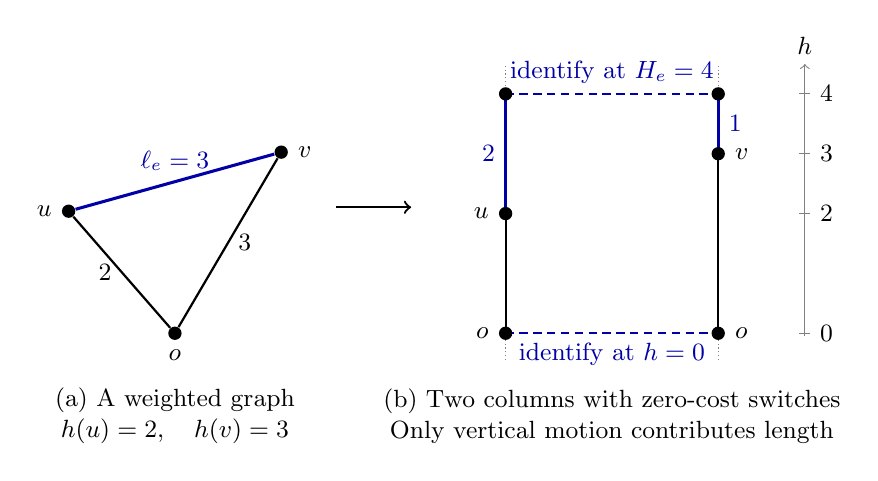
\begin{tikzpicture}[x=1cm,y=1cm,font=\small,
  vertex/.style={circle,fill=black,inner sep=1.7pt},
  twig/.style={blue!65!black,line width=1.1pt},
  identify/.style={blue!65!black,densely dashed,line width=.8pt}]
  \node[vertex,label=below:$o$] (o) at (0,0) {};
  \node[vertex,label=left:$u$] (u) at (-1.35,1.55) {};
  \node[vertex,label=right:$v$] (v) at (1.35,2.3) {};
  \draw[thick] (o)--node[left] {$2$} (u);
  \draw[thick] (o)--node[right] {$3$} (v);
  \draw[twig] (u)--node[above] {$\ell_e=3$} (v);
  \node[align=center] at (0,-1.05) {(a) A weighted graph\\$h(u)=2,\quad h(v)=3$};

  \draw[->,thick] (2.05,1.6)--(3,1.6);

  \begin{scope}[shift={(4.2,0)},y=.76cm]
    \draw[gray,densely dotted] (0,-.45)--(0,0);
    \draw[gray,densely dotted] (2.7,-.45)--(2.7,0);
    \draw[thick] (0,0)--(0,2);
    \draw[thick] (2.7,0)--(2.7,3);
    \draw[twig] (0,2)--node[left] {$2$} (0,4);
    \draw[twig] (2.7,3)--node[right] {$1$} (2.7,4);
    \draw[gray,densely dotted] (0,4)--(0,4.5);
    \draw[gray,densely dotted] (2.7,4)--(2.7,4.5);
    \draw[identify] (0,0)--node[below] {identify at $h=0$} (2.7,0);
    \draw[identify] (0,4)--node[above] {identify at $H_e=4$} (2.7,4);
    \node[vertex,label=left:$o$] at (0,0) {};
    \node[vertex,label=right:$o$] at (2.7,0) {};
    \node[vertex,label=left:$u$] at (0,2) {};
    \node[vertex,label=right:$v$] at (2.7,3) {};
    \node[vertex] at (0,4) {};
    \node[vertex] at (2.7,4) {};
    \draw[->,gray] (3.8,-.05)--(3.8,4.5) node[above,black] {$h$};
    \foreach \h in {0,2,3,4} {
      \draw[gray] (3.73,\h)--(3.87,\h) node[right,black] {$\h$};
    }
  \end{scope}
  \node[align=center] at (5.55,-1.05) {(b) Two columns with zero-cost switches\\Only vertical motion contributes length};
\end{tikzpicture}
\caption{An exact example of Proposition~\ref{geo:realization}.
The black edges form a shortest-path tree rooted at $o$.
The non-tree edge is replaced by two ascending twigs of lengths
$(\ell_e+h(v)-h(u))/2=2$ and $(\ell_e+h(u)-h(v))/2=1$.
Their tips have the same height $H_e=4$ and are identified.
Dashed horizontal segments denote identifications, not extra edges;
the dotted vertical tails do not shorten original distances.}
\label{fig:column-realization}
\end{figure}


\subsection{Consequences of the circular order}

The circular order gives separation statements used later for ordered
fields and the seed packing argument. These statements concern the column
graph, so they hold simultaneously for all height bands. Its outerplanarity
will also give the two-portal estimate in the next subsection.

\begin{lemma}[Chord separation]\label{geo:chord-separation}
Let $uv$ be an edge of a noncrossing circular graph.  Any graph path from
the strict interior of one circular $u$--$v$ arc to the strict interior of
the other visits $u$ or $v$.
\end{lemma}

\begin{proof}
A path avoiding $u,v$ and changing arcs has an edge whose endpoints lie
in the two strict interiors.  Its endpoints alternate with $u,v$, which
contradicts noncrossing.
\end{proof}

\begin{lemma}[Gaps of a connected set]\label{geo:gap}
Let $S$ be a nonempty connected vertex set in a noncrossing circular graph.
Every graph path avoiding $S$ lies in one of the open circular gaps between
consecutive vertices of $S$.  Here the complement of a singleton is regarded
as one gap.  Connectivity of $S$ and the path may be witnessed using
different subgraphs of the same noncrossing graph.
\end{lemma}

\begin{proof}
Suppose an edge $uv$ of the path joined distinct gaps.  Then each strict
circular $u$--$v$ arc contains a vertex of $S$.  A path inside $S$ joining
these two vertices would have to visit $u$ or $v$ by
Lemma~\ref{geo:chord-separation}.  Both endpoints lie outside $S$, a
contradiction.  Thus each edge stays in one gap, and so does the whole path.
\end{proof}

\begin{lemma}[Skipping a column]\label{geo:skipping}
Give an open circular arc its linear order, and assume its complementary
closed arc contains a column index.  Let a vertex walk stay in the open
arc, and let an index $i$ lie strictly between its initial and final indices.
Either the walk visits $i$, or one of its edges has endpoints strictly on
opposite sides of $i$.  In the latter case the edge is a non-neighbor link.
If a second path starts strictly between the endpoints of this edge and
leaves that strict interval, it visits an endpoint of the edge.
\end{lemma}

\begin{proof}
If the walk avoids $i$, take its first edge changing from one side of $i$
to the other.  The index $i$ lies on one strict circular arc between its
endpoints, and an index in the complementary closed arc lies on the other.
They are therefore not cyclic neighbors.  The final assertion is
Lemma~\ref{geo:chord-separation}.
\end{proof}

\begin{lemma}[Outerplanarity]\label{geo:outerplanar}
Every active graph $G_I$ is outerplanar and has no $K_{2,3}$ minor.
\end{lemma}

\begin{proof}
Place the indices on a circle and draw each edge as a straight chord.
The noncrossing condition makes this an outerplanar drawing.  Add a new
vertex in the complementary disk on the sphere and join it to every
column vertex by a disjoint radial star.  The resulting cone graph is
planar.  If $G_I$ had a $K_{2,3}$ minor, perform its deletions and contractions
while retaining the new vertex and one edge from it to every contracted
branch set.  The resulting planar minor contains the cone over $K_{2,3}$.
That cone contains $K_{3,3}$: add the cone vertex to the part of size two.
This is impossible, since a simple bipartite planar graph on six vertices
has at most eight edges, whereas $K_{3,3}$ has nine.
\end{proof}

\begin{lemma}[Connected distance sublevels]\label{geo:sublevel}
Fix a component of $X_I$, a source $o$ in it, and a height $H\in I$.
Put $q_i=d_I(o,(i,H))$, taking $q_i=+\infty$ outside that component.
For every real $t$, the nonempty set $\{i:q_i\le t\}$ is connected in
$G_I$.
\end{lemma}

\begin{proof}
For an index $i$ in the set, take a shortest path from $o$ to $(i,H)$.
If it visits a column $j$ at height $H'$, stop there and move vertically
to $(j,H)$.  The cost of this new ending is $|H-H'|$, at most the vertical
variation of the discarded suffix.  Thus $q_j\le q_i\le t$.  The projected
path therefore lies in the sublevel set and joins $i$ to the source column.
Taking these paths for all $i$ proves connectivity.  This argument also
shows that every source-column representative belongs to the sublevel
whenever the sublevel is nonempty.
\end{proof}

\subsection{Portals and radial cells}

We will cover the entrances to a connected radial superlevel set by at
most two controlled balls.  This estimate will then bound distances
within the connected pieces of each radial layer.

In this subsection $J$ is a closed band of width $a>0$, $H_*$ is its
midheight, and we work in a fixed component of $X_J$.  Choose a basepoint
$o$ and define
\[
 b_i=d_J(o,(i,H_*)).
\]
For a point $v=(i,H)$ in the band,
\begin{equation}\label{geo:radial-estimates}
 \bigl|d_J(o,v)-b_i\bigr|\le a/2,
 \qquad |b_i-b_j|\le a\quad\text{if }ij\in G_J.
\end{equation}
The second estimate follows by traveling from the two midpoints to an
available switch, at cost at most $a$.  We occasionally use the weaker
bound $2a$ without further comment.

\begin{lemma}[Two portals]\label{geo:portals}
Let $C$ be a component of the subgraph of $G_J$ induced by $\{i:b_i\ge t\}$.
An \emph{entrance column} of $C$ is an index in $C$ adjacent to an index
with radial value below $t$.  If entrance columns exist, there are at most
two of their midpoints, called portals, such that every point on every
entrance column lies within $200a$ in $d_J$ of one of the portals.
Every portal has radial value in $[t,t+a)$.  If $t>a/2$ and $C$ is nonempty,
entrance columns exist.
\end{lemma}

\begin{proof}
An entrance column has $t\le b_i<t+a$ by
\eqref{geo:radial-estimates}.  When $t<30a$, all entrance midpoints have
distance less than $31a$ from $o$.  Any one is therefore within $62a$ of
every other, and within $63a$ of every point on every entrance column.
One portal suffices in this case.

Suppose $t\ge30a$.  Let $L$ be the projection to columns of the closed
ball $B_{d_J}(o,t-12a)$.  Shortest paths from $o$ to the points
of the ball stay in the ball, so $L$ is connected.  Every $j\in L$ has
$b_j\le t-12a+a/2$, and hence $L$ is disjoint from $C$.

Assume there are three entrance midpoints $x_1,x_2,x_3$ at pairwise
distance greater than $100a$.  Starting from each $x_k$, follow a shortest
path toward $o$ until its first visit to a column of $L$.  This portion
has length at most $13a$: by that length it reaches a point at radial
distance $t-12a$.  Its projection joins $C$ to $L$.  The three projected
portions are vertex-disjoint.  Indeed a common column would permit a
vertical transfer of length at most $a$, giving a path of length at most
$13a+a+13a<100a$ between the corresponding entrance points.

For each portion retain the segment after its last visit to $C$ and
before its first visit to $L$.  Its interior avoids both sets.  It has
an internal vertex, since its endpoints have radial values differing by
at least $12a-a/2>a$, while adjacent columns differ by at most $a$.
Contract the connected sets $C$ and $L$, and contract each of the three
nonempty connector interiors to a separate vertex.  This gives a
$K_{2,3}$ minor, contrary to Lemma~\ref{geo:outerplanar}.

A maximal set of entrance midpoints at mutual distances greater than
$100a$ thus has cardinality at most two.  Maximality covers every entrance
midpoint within $100a$, and the extra vertical distance is at most $a/2$.
This proves the stated $200a$ bound.  Finally a representative of $o$ has
radial value at most $a/2$.  If $t>a/2$, any nonempty high component is a
proper subset of the connected graph and has an entrance.
\end{proof}

\begin{figure}[tbp]
\centering
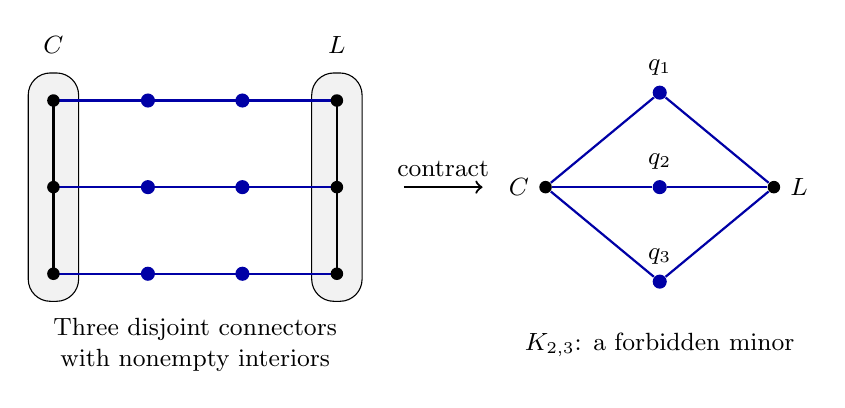
\begin{tikzpicture}[x=1cm,y=1cm,font=\small,
  vertex/.style={circle,fill=black,inner sep=1.6pt},
  interior/.style={circle,fill=blue!65!black,inner sep=1.8pt}]
  \draw[fill=gray!10,rounded corners=8pt] (-.32,-1.45) rectangle (.32,1.45);
  \draw[fill=gray!10,rounded corners=8pt] (3.28,-1.45) rectangle (3.92,1.45);
  \draw[thick] (0,-1.1)--(0,1.1);
  \draw[thick] (3.6,-1.1)--(3.6,1.1);
  \foreach \y in {-1.1,0,1.1} {
    \draw[blue!65!black,thick] (0,\y)--(3.6,\y);
    \node[vertex] at (0,\y) {};
    \node[vertex] at (3.6,\y) {};
    \node[interior] at (1.2,\y) {};
    \node[interior] at (2.4,\y) {};
  }
  \node at (0,1.8) {$C$};
  \node at (3.6,1.8) {$L$};
  \node[align=center] at (1.8,-2) {Three disjoint connectors\\with nonempty interiors};
  \draw[->,thick] (4.45,0)--(5.45,0) node[midway,above] {contract};

  \node[vertex,label=left:$C$] (C) at (6.25,0) {};
  \node[vertex,label=right:$L$] (L) at (9.15,0) {};
  \foreach \y/\k in {1.2/1,0/2,-1.2/3} {
    \node[interior,label=above:$q_\k$] (q\k) at (7.7,\y) {};
    \draw[blue!65!black,thick] (C)--(q\k)--(L);
  }
  \node at (7.7,-2) {$K_{2,3}$: a forbidden minor};
\end{tikzpicture}
\caption{The hypothetical obstruction in Lemma~\ref{geo:portals}.
Three sufficiently separated entrance points would give vertex-disjoint
paths from the connected high set $C$ to the connected low set $L$.
After trimming, each connector has a nonempty interior avoiding both
sets. Contracting $C$, $L$, and the three interiors gives $K_{2,3}$,
which cannot be a minor of the outerplanar column graph.
The drawing records this contraction; it is not an outerplanar drawing
of a configuration that the column model permits.}
\label{fig:two-portals}
\end{figure}


\begin{definition}[Radial cells]\label{geo:cell-definition}
Fix $D>0$ and an offset $\theta\in[0,D)$.  Partition the indices into
layers by assigning $i$ to the unique half-open interval
\[
 [\theta+nD,\theta+(n+1)D),\qquad n\in\mathbb Z,
\]
containing $b_i$.  Split each layer into the connected components of its
induced subgraph of $G_J$.  A \emph{cell} is the image in $X_J$ of all
intervals $\{i\}\times J$ belonging to one such component. Its
\emph{frontier} $\partial C$ is the union of their images for indices
adjacent in $G_J$ to an index outside the cell.
\end{definition}

This is a partition of the column indices, not necessarily a disjoint
partition of their quotient images.  If two cells share a quotient point,
that point belongs to the frontier of each: a switch chain identifying
representatives in the two cells has a first edge leaving either cell.
Consequently formulas that agree with the unchanged data on all frontiers
give unambiguous values at such shared points.

Here a \emph{weak diameter} bound measures distances in the whole band;
the paths witnessing those distances may leave the cell.

\begin{lemma}[Diameter of cells]\label{geo:cells}
Assume $a\le D/1000$.  Every radial cell is compact and path-connected,
and has weak diameter at most $10D$ in $d_J$.  Its frontier is compact,
possibly empty.
\end{lemma}

\begin{proof}
Each cell is the image of finitely many closed column intervals.  Its
column graph is connected, which makes that image path-connected.  The
same finite-union argument proves compactness of the cell and frontier.

Let $q$ be the lower threshold of its layer.  If $q\le30a$, every point
of the cell has distance less than $D+31a$ from $o$, so the diameter bound
follows.  Suppose $q>30a$ and let $C^+$ be the component of $\{b_i\ge q\}$
containing the cell.  It has at most two entrance portals by
Lemma~\ref{geo:portals}.

Take $v$ in the cell and follow a shortest path to $o$ until the first
switch below threshold $q$.  Before that switch the projected path stays
in $C^+$: two adjacent high columns belong to the same high component.
The last high column is an entrance, and the switch point has radial
distance at least $q-a/2$.  Since $d_J(o,v)<q+D+a/2$, the portion from $v$
to that point has length less than $D+a$.  Some portal is within $200a$
of that point.  Thus the cell is contained in the union of two closed
balls of radius $D+210a$ around its portals.

A connected set contained in the union of two closed balls either lies
in one of them or meets their intersection.  To see the second alternative
when neither ball contains the set, intersect both balls with the connected
set; two nonempty disjoint closed subsets could not cover it.  In that
case the centers have distance at most $2(D+210a)$.  In either alternative
the cell has diameter at most $4(D+210a)<10D$.
\end{proof}

\begin{lemma}[Padding and separation of cell interiors]\label{geo:padding}
Let $v=(i,H)\in X_J$, and let $T=\theta+D\mathbb Z$ be the radial
threshold set.  If
\begin{equation}\label{geo:padding-condition}
 \dist(b_i,T)>\rho+2a,
\end{equation}
then every point reachable from $v$ by a band path of length at most
$\rho$ has all its representatives in the same cell as $i$.  Moreover
$d_J(v,\partial C)>\rho$ for that cell.

For uniform $\theta\in[0,D)$, the probability that
\eqref{geo:padding-condition} fails is at most
\[
 \min\{1,\,2(\rho+2a)/D\}.
\]
There is no factor for the number of representatives of $v$: their
radial values differ pairwise by at most $a$.

In particular, if $a\le D/1000$ and the radial values of two points are
at distance greater than $0.02D$ from the thresholds, then their distances
to their respective frontiers are greater than $0.01D$.  If they belong
to different cells, their mutual $d_J$-distance is greater than $0.01D$.
\end{lemma}

\begin{proof}
If a band path from $v$ of length at most $\rho$ visits column $k$, join
its visit point to $(k,H_*)$ and join $v$ to $(i,H_*)$.  The triangle
inequality gives
\[
 |b_k-b_i|\le\rho+a.
\]
Thus every visited column stays in $i$'s layer under
\eqref{geo:padding-condition}; its projected path puts it in the same
connected component of that layer.  The same argument applies after any
zero-cost switch chain at an endpoint, proving the assertion about all
representatives.

Every frontier column has its radial value within $a$ of one of the
cell's layer thresholds: its neighbor outside the cell cannot belong
to the same layer.  If $z$ lies on a frontier column $k$, then
\[
 d_J(v,z)\ge |b_i-b_k|-a
       \ge \dist(b_i,T)-2a>\rho.
\]
The formula remains true for an empty frontier with distance $+\infty$.
The offset estimate is the length, at most $2(\rho+2a)$, excluded in one
period.  Two representatives at height $H$ have midpoint distance at
most $2|H-H_*|\le a$, since their points at height $H$ are identical.
This proves the representative assertion without a union bound.

For the numerical conclusion use
$0.02D-2a\ge0.018D>0.01D$.  A path to a different cell must first visit
a frontier column of the initial cell, so the same lower bound applies
to its length.
\end{proof}

The cell estimates will control the regions where the local updates act.
For interpolation we also need the entrance estimate at successive radial
thresholds. The resulting components form a rooted tree, with controlled
distances between the portals at successive levels.

\begin{lemma}[Successive portal levels]\label{geo:portal-levels}
Fix a step $\delta>1000a$.  At depth $n\ge1$ take the components of
$\{b_i\ge n\delta\}$ and give each its entrance portals from
Lemma~\ref{geo:portals}.  The depth-zero node is the whole component,
with its sole portal $o$.  Each positive-depth node has a unique parent.
For a node at depth $n$, every point on one of its columns with
$b_i<(n+1)\delta$, and every portal of one of its children, is within
$\delta+220a$ of one of its own portals.  Each child portal is at distance
at least $\delta-10a$ from every own portal.
\end{lemma}

\begin{proof}
A connected component at a higher threshold is contained in a unique
component at the preceding threshold, proving the parent assertion.
For $n\ge1$, repeat the root-geodesic argument in
Lemma~\ref{geo:cells} at lower threshold $n\delta$.  A point of the
node's own layer has radial distance below $(n+1)\delta+a/2$.  A child
portal has radial distance in
$[(n+1)\delta,(n+1)\delta+a)$.  In either case its geodesic reaches an
entrance of the parent node after length at most $\delta+2a$, and an
own portal is within a further $200a$.  The asserted upper bound follows.

An own portal has radial distance in $[n\delta,n\delta+a)$, whereas a
child portal has radial distance at least $(n+1)\delta$.  Their distance
is therefore at least $\delta-a$.  At depth zero the upper bounds follow
directly by taking $o$, and a depth-one portal is at distance at least
$\delta$ from it.  These estimates imply the stated bounds in every case.
\end{proof}
